\documentclass[]{article}

%format
\usepackage[utf8]{inputenc}
\usepackage[T1]{fontenc}
\usepackage[english]{babel}
\usepackage[margin=2.5cm]{geometry}
%math
\usepackage{amsthm}
\usepackage{amsmath}
\usepackage{amsfonts}
\usepackage{amssymb}
\usepackage{stmaryrd}
\usepackage{nicefrac}
\usepackage{mathtools}
%others
\usepackage{hyperref}
\usepackage{graphicx}
\usepackage{enumitem}

%environments
\newtheorem{question}{Question}
%commands
%\newcommand{\name}[num]{definition}
\newcommand{\primes}{\mathbb{P}}
%\newcommand{\P}{\mathbb{P}}
\newcommand{\N}{\mathbb{N}}
\newcommand{\Z}{\mathbb{Z}}
\newcommand{\Q}{\mathbb{Q}}
\newcommand{\D}{\mathbb{D}}
\newcommand{\R}{\mathbb{R}}
\newcommand{\C}{\mathbb{C}}
\newcommand{\F}{\mathbb{F}}
\newcommand{\B}{\mathbb{B}}
\newcommand{\Norm}[2][]{\text{Norm}_{#1}(#2)}
\newcommand{\inner}[2]{\left\langle #1,#2 \right\rangle}
\newcommand{\floor}[1]{\lfloor #1 \rfloor}
\newcommand{\ceil}[1]{\lceil #1 \rceil}
\newcommand{\abs}[1]{| #1 |}
\newcommand{\card}[1]{| #1 |}
\newcommand{\curt}[1]{\sqrt[3]{#1}}
\newcommand{\Ker}[1]{\text{Ker}(#1)}
\newcommand{\Image}[1]{\text{Im}(#1)}
\newcommand{\Trace}[1]{\text{Tr}(#1)}
\newcommand{\Det}[1]{\text{Det}(#1)}
\newcommand{\degree}[1]{\partial #1}
\newcommand{\Pow}[1]{\mathcal{P}(#1)}

%opening
\title{Problem Set 1}
\author{}
\date{Due 9\textsuperscript{th} September 2021}

\begin{document}

\maketitle

\begin{abstract}
	Only the questions with a star (*) are compulsory for submission;\\
	It is however \textit{strongly} advised to attempt all question.
\end{abstract}

\section{Sets \& Logic}
\subsection{Sets}

\begin{figure}[h!]
	\centering
	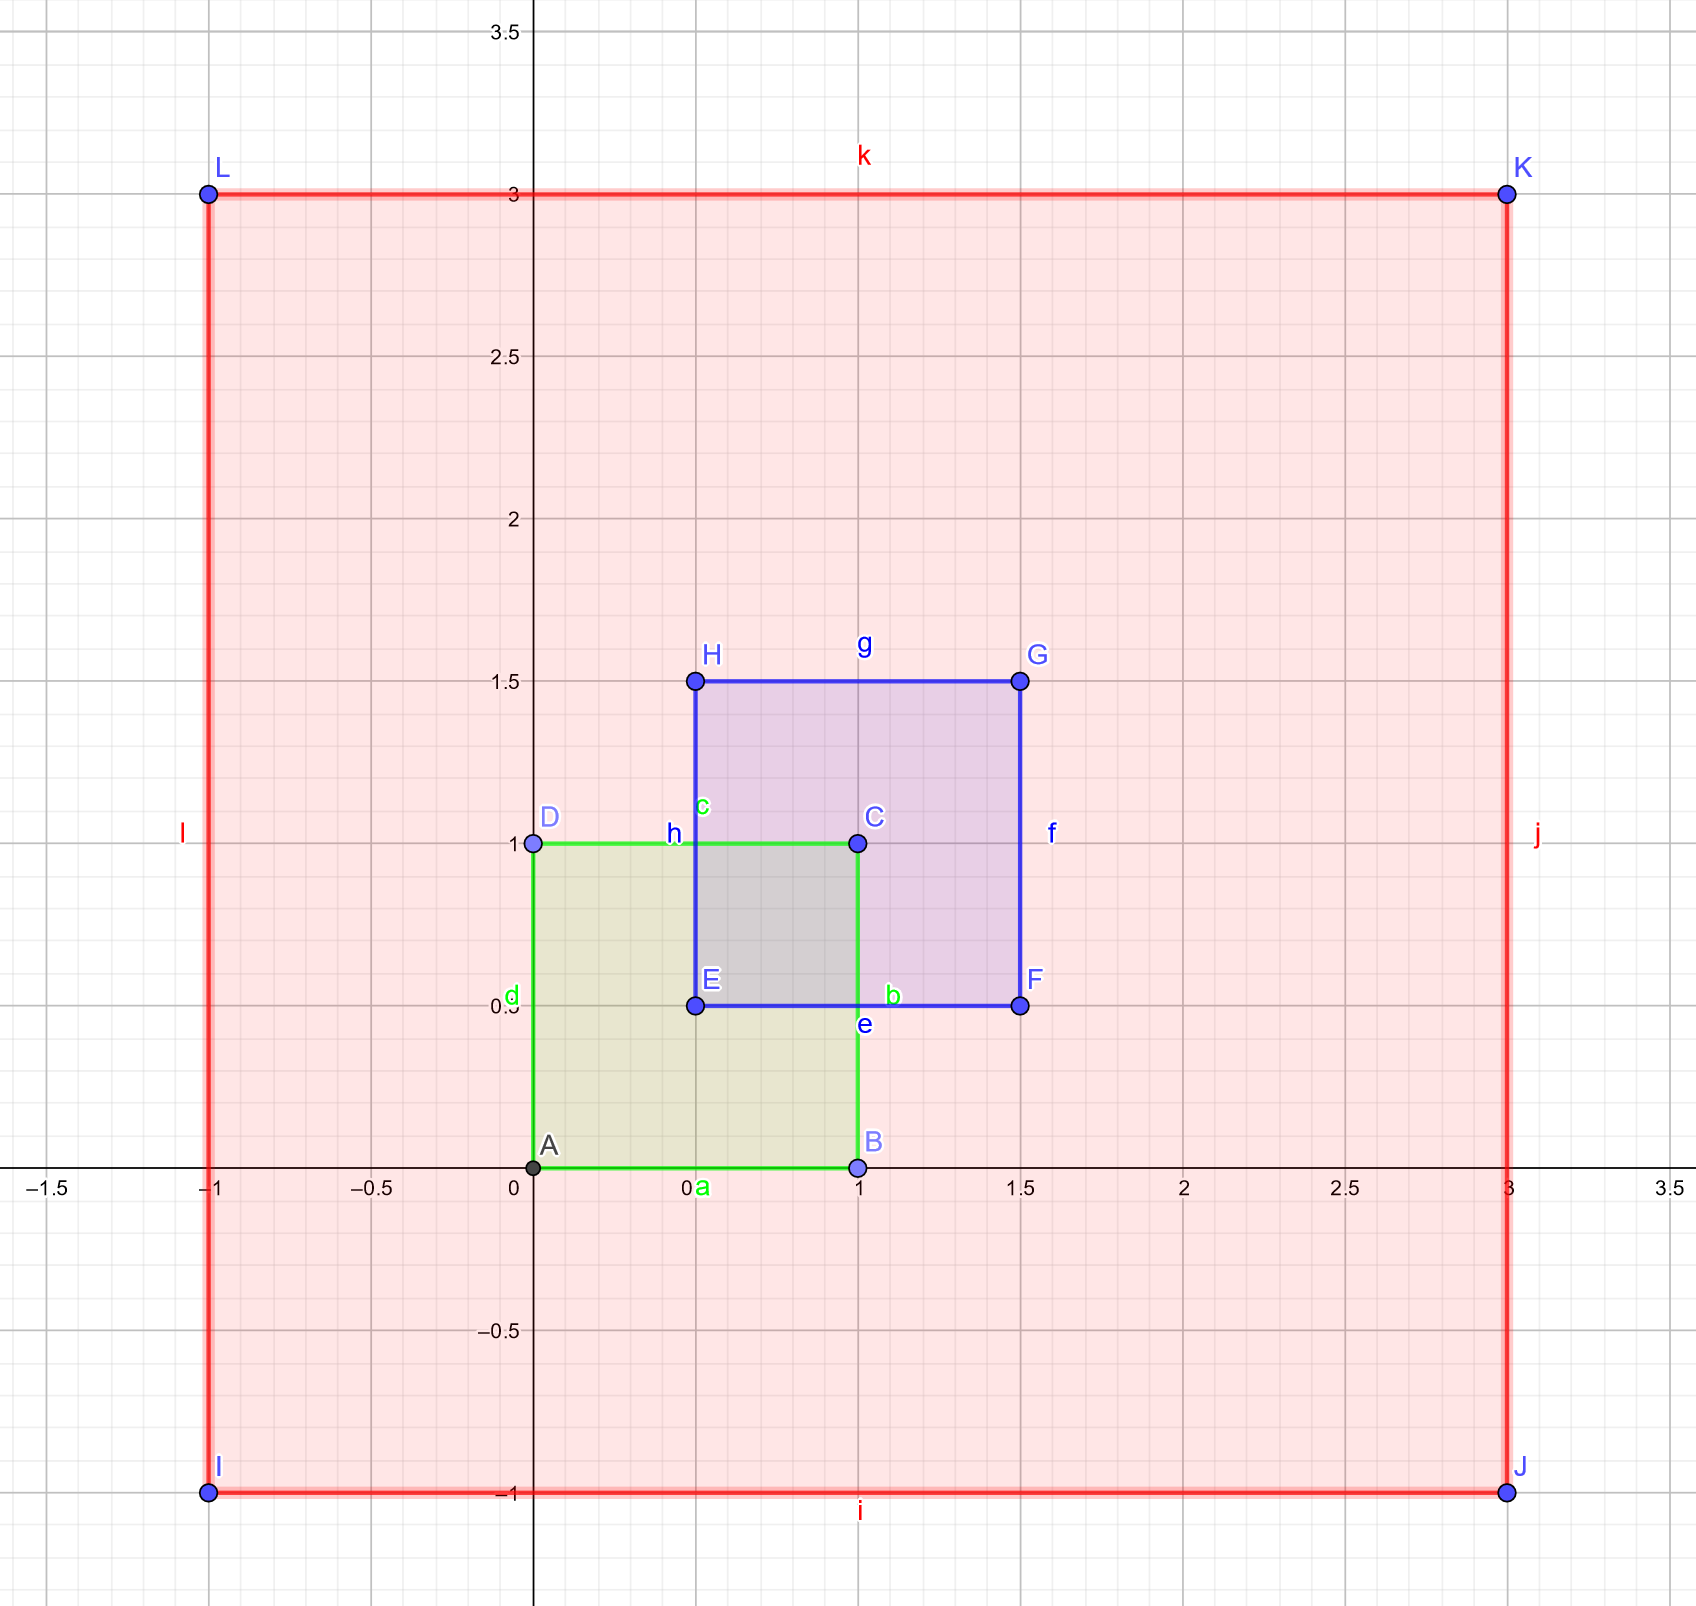
\includegraphics[width=0.6\textwidth]{1-sets.png}
\end{figure}
\begin{question}[*]
	We call $R$ the set of points in the red square, $B$ for the ones in the blue square, and $G$ for the green one.
	\begin{enumerate}[label=\alph*.]
		\item Express $R$, $G$, and $B$ in terms of Cartesian product.\footnote{$G$ is in fact called the unit square in the first quadrant.}
		\item Give all (if any) the subsets relations between $R$, $G$, and $B$.
		\item Express $G \cup B \setminus (G \cap B)$ in terms of Cartesian product.
		\item Express $\left[ 1/2,1 \right]^2$ in terms of $R$, $G$, and $B$ (using intersections, unions, ...).
		\item Express $\left[ 1/2,3/2 \right] \times \left[ 1,3/2 \right] \cup \left[ 1,3/2 \right] \times \left[ 1/2,3/2 \right]$ in terms of $R$, $G$, and $B$.
	\end{enumerate}
\end{question}

\begin{figure}[h!]
	\centering
	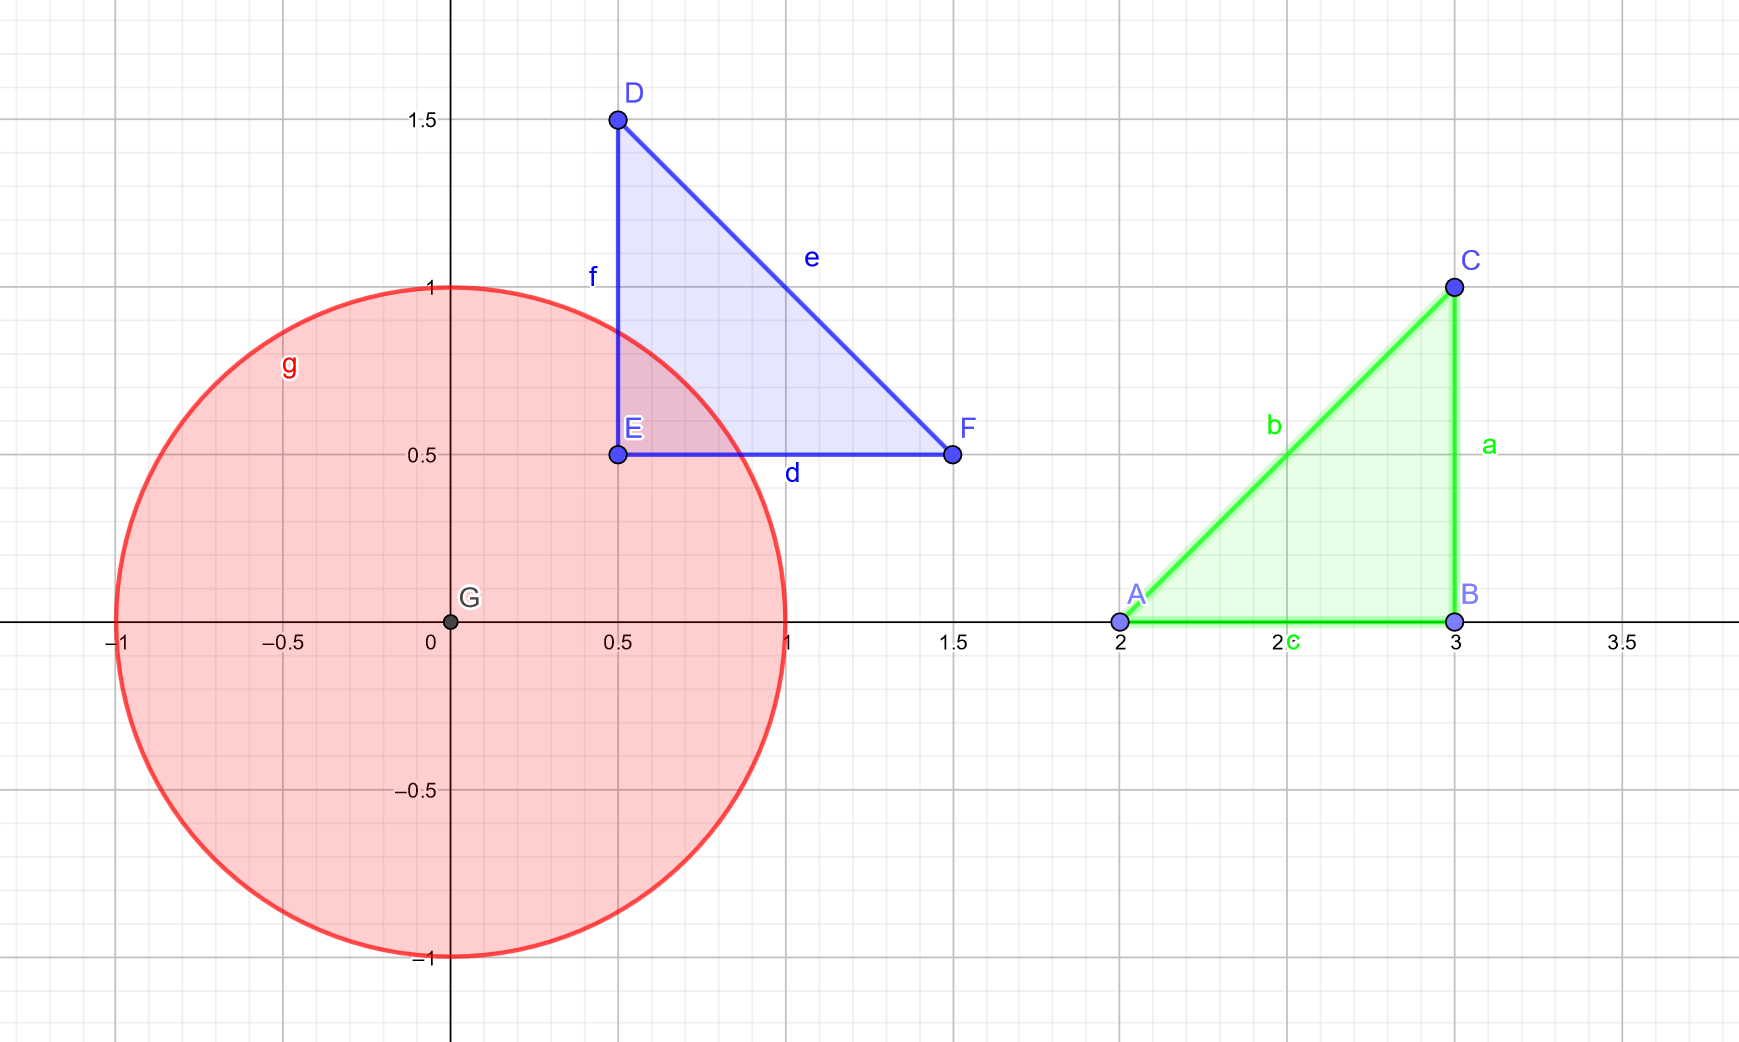
\includegraphics[width=0.6\textwidth]{2-sets.png}
\end{figure}
\begin{question}
	We call $R$ the set of points in the red disc, $B$ for the ones in the blue triangle, and $G$ for the green one.
	\begin{enumerate}[label=\alph*.]
		\item (*) Express $R$, $G$, and $B$ using set notation with predicates (i.e. $\{ object \mid condition \}$) of Cartesian product.\footnote{$R$ is in fact called the unit disc.}
		\item Express $R \cap B$ using set notation.
		\item (*) Draw $R \cap \{ (x,y) \mid x \leq 0, y \leq 0 \}$.
		\item The upper half plane $\mathcal{H}$ is $\{ (x,y) \mid y>0 \}$; hatch it on your figure.
		\item Which one(s) (if any) of $R$, $G$, $B$ is contained in $\mathcal{H}$?
	\end{enumerate}
\end{question}

\subsection{Boolean Algebra}
\begin{question}
	Here, $a,b,c,d \in \B$ are boolean numbers.
	\begin{enumerate}[label=\alph*.]
		\item (*) Show that $abc+\overline{a}bc+a\overline{b}c+ab\overline{c}=bc+ac+ab$
		\item (*) Check that $abc+\overline{a}bc+a\overline{b}c+ab\overline{c}=bc+ac+ab$ using truth tables
		\item Show that $abc+ab\overline{c}+a\overline{b}cd=ab+acd$
	\end{enumerate}
\end{question}
\begin{question}
	Here again, $a,b,c \in \B$ are boolean numbers. One wants to add them, and display the result in base 2 using two LEDs (one for the units, one for the twos).
	The complete truth table is given below; find expressions for the units and twos.
\end{question}
\begin{figure}[h!]
	\begin{center}
		\begin{tabular}{ c c c | c | c }
			$a$ & $b$ & $c$ & tows of $a+b+c$ & units of $a+b+c$ \\
			\hline
			0 & 0 & 0 & 0 & 0\\  
			0 & 0 & 1 & 0 & 1\\
			0 & 1 & 0 & 0 & 1\\  
			0 & 1 & 1 & 1 & 0\\
			1 & 0 & 0 & 0 & 1\\  
			1 & 0 & 1 & 1 & 0\\
			1 & 1 & 0 & 1 & 0\\  
			1 & 1 & 1 & 1 & 1\\
		\end{tabular}
	\end{center}
\end{figure}

\subsection{Quantified propositions}
\begin{question}[*]
	Negate the following\footnote{This is in fact the definition of $x_n$ converging to $x$ ($x_n \to x$).}:
	$\forall \epsilon>0, \exists N \in \N \text{ s.t. } \forall n>N, \abs{x_n-x}<\epsilon$
\end{question}
\begin{question}
	Find the quantified notation of the following sentences:
	\begin{enumerate}[label=\alph*.]
		\item (*) "Given a number, it always possible to find another one that is greater"
		\item (*) "Any natural number is non-negative"
		\item "There is no negative square"\footnote{(in the reals)}
		\item "There exists a bijection between the naturals and the set of all fractions"
	\end{enumerate}
\end{question}

\section{Modular Arithmetic}
\textit{This is not needed for the rest of the course, but is nice to know}
Read the first two sections of \url{https://en.wikipedia.org/wiki/Modular_arithmetic}.
\begin{question}
	\begin{enumerate}[label=\alph*.]
		\item Show that $n^2$ is divisible by 3 if and only if $n$ is divisible by 3.
		\item Show that $n^2$ is divisible by 5 if and only if $n$ is divisible by 5.
		\item (harder) Show that $n^2$ is divisible by $p$ if and only if $n$ is divisible by $p$ for any prime $p$.\footnote{Hint: look for Euclid's lemma.}
	\end{enumerate}
\end{question}


\section{Proofs Methods}
\begin{question}
	\begin{enumerate}[label=\alph*.]
		\item (*) Show that $n$ divisible by 6 if and only if $n$ divisible by 2 and 3.
		\item Show $\sqrt{3} \not\in \Q$.\footnote{See congruence on Wikipedia}
		\item Show that $12N-6$ is divisible by 6 for every positive integer $n$.
		\item Show that $2^n \geq 2n$ for all $n \in \N$
	\end{enumerate}
\end{question}


\section{Functions Properties}
\begin{question}
	\begin{enumerate}[label=\alph*.]
		\item (*) $f: X \to Y, \ g: Y \to Z \text{ injectives } \implies g \circ f \text{ is injective}$\\
		\item $f: X \to Y, \ g: Y \to Z \text{ surjectives } \implies g \circ f \text{ is surjective}$\\
		\item $f: X \to Y, \ g: Y \to Z \text{ bijectives/invertibles } \implies g \circ f \text{ is bijective/invertible}$
	\end{enumerate}
\end{question}







\end{document}
